\documentclass[12pt]{article}

\usepackage{amsmath, amsthm, amssymb, amsbsy, amsfonts}
\usepackage[plainpages=false,pdfpagelabels]{hyperref}
\hypersetup{
    colorlinks,
    citecolor=black,
    filecolor=black,
    linkcolor=black,
    urlcolor=blue
}
\usepackage{verbatim}
\usepackage{enumitem}
\usepackage[utf8x]{inputenc}

% Redefine the \vec command to use bold font instead of an arrow
\renewcommand\vec[1]{\mathbf{#1}}

%\def\nl{\hfill\break\null}
\oddsidemargin=0.3cm
\topmargin=-1cm
\textwidth=15cm
\textheight=23cm
\parindent=0cm
\parskip=1mm


\usepackage{graphicx}
\DeclareMathOperator*{\argmin}{argmin}

\newenvironment{enumialpha}{\begin{enumerate}
  \def\theenumi{\alph{enumi}}
  \def\labelenumi{(\theenumi)}}{\end{enumerate}}

\newenvironment{enumiiroman}{\begin{enumerate}
  \def\theenumii{\roman{enumii}}
  \def\labelenumii{(\theenumii)}}{\end{enumerate}}


\begin{document}

\begin{tabular*}{15cm}{@{}l@{\extracolsep{\fill}}r}
  Albert-Ludwigs-Universit\"at Freiburg, Institut f\"ur Informatik \\
PD Dr. Cyrill Stachniss \\  Lecture: Robot Mapping \\
  Winter term 2013 
\end{tabular*}

\bigskip


\begin{center}
  {\bf \Large Sheet 7}

  {\large Topic: Grid Maps}

  Submission deadline: December, 16\\
  Submit to: \texttt{robotmappingtutors@informatik.uni-freiburg.de}
\end{center}

\subsubsection*{Exercise: Occupancy Mapping Algorithm Implementation}

Implement the occupancy grid mapping algorithm as presented in the
lecture. To support this task, we provide a small \emph{Octave} framework (see
course website).  The framework contains the following folders:

\begin{description}
  \item [data]
    contains the recorded laser scans and known robot poses at each time step.
  \item [octave]
    contains the grid maps framework with stubs to complete.
  \item [plots]
    this folder is used to store images.
\end{description}

The below mentioned tasks should be implemented inside the framework in
the directory \texttt{octave} by completing the stubs:

\begin{itemize}
  \item
    Implement the functions in \texttt{prob\_to\_log\_odds.m} and
    \texttt{log\_odds\_to\_prob.m} for converting between probability
    and log odds values.
  \item
    Implement the function in \texttt{world\_to\_map\_coordinates.m} for
    converting the $(x,y)$ world frame coordinates of a point to its
    corresponding coordinates in the grid map. You might find the
    \emph{Octave} functions \texttt{ceil} and \texttt{floor} useful.
  \item
    Implement the function in \texttt{inv\_sensor\_model.m} to compute
    the update to the log odds value of each cell in the map for a
    particular laser scan measurement.
\end{itemize}

After implementing the missing parts, you can run the occupancy grid
mapping framework.  To do that, \textbf{change into the directory
octave} and launch \emph{Octave}.  Type \texttt{gridmap} to start the
main loop (this may take some time).  The script will produce plots of
the state of the resulting maps and save them in the \texttt{plots}
directory.  You can use the images for debugging and to generate an
animation. For example, you can use ffmpeg from inside the plots
directory as follows:
\begin{verbatim}
ffmpeg -r 10 -b 500000 -i gridmap_%03d.png gridmap.mp4
\end{verbatim}

\begin{figure}
  \centering
  \begin{tabular}{cc}
    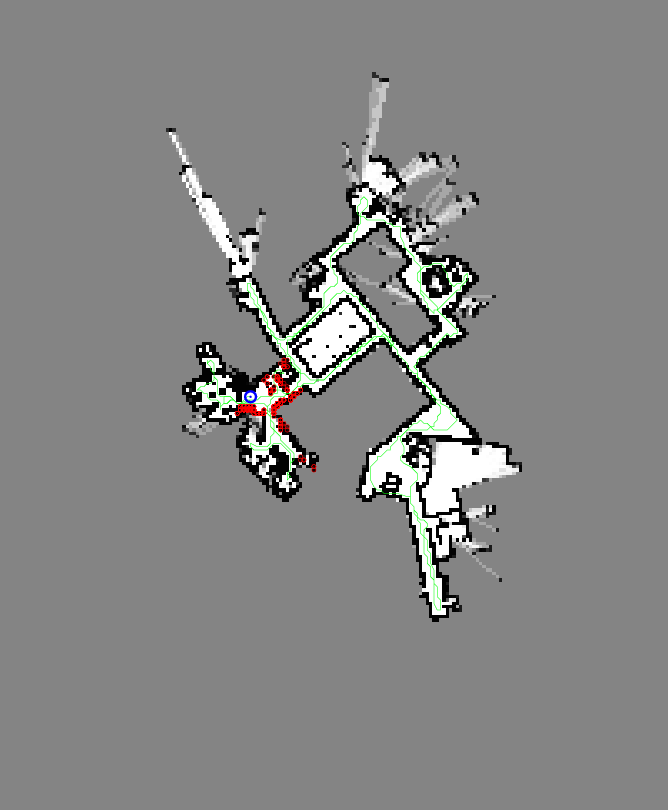
\includegraphics[height=7cm]{gridmap_0_5.png} &
    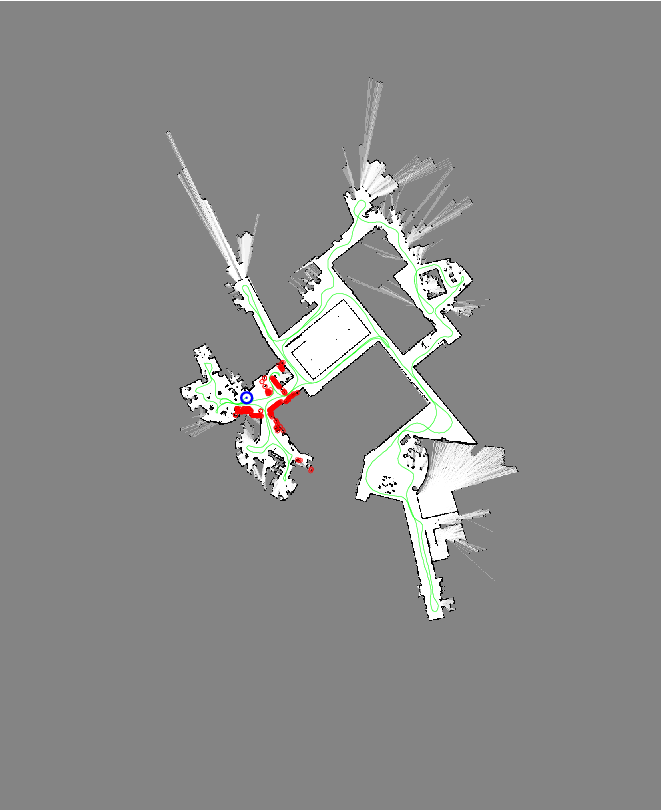
\includegraphics[height=7cm]{gridmap_0_1.png}\\
    resolution 0.5\,m & resolution 0.1\,m
  \end{tabular}
  \caption{Examples for the final result of the occupancy mapping algorithm.}
  \label{fig:examples}
\end{figure}

Figure~\ref{fig:examples} depicts the example images of the resulting
maps using grid sizes of 0.5\,m and 0.1\,m.

Some implementation tips:
\begin{itemize}
  \item Use an inverse sensor model corresponding to laser range finders
    (see lecture slides). The corresponding $p_{free}$ and $p_{occ}$
    values are specified in the \texttt{gridmap.m} script. Use $p_{occ}$
    to update the occupancy value of cells that laser beam endpoints hit
    and $p_{free}$ for all other cells along the beam. Use the function
    \texttt{robotlaser\_as\_cartesian.m} to compute the Cartesian
    coordinates of the endpoints of a laser scan. The provided
    \texttt{bresenham.m} function can be used for computing the cells
    that lie along a laser beam in map coordinates.
  \item
    Compute all occupancy value updates in log odds (not probabilities)
    so they can be added directly to the map.
  \item
    Test your implementation with a grid size of 0.5m. Once you are
    satisfied with your results, you can run the algorithm with an
    increased resolution (e.g. 0.1m), as this will take considerably
    more time.
  \item
    While debugging, run the algorithm only for a few steps by
    replacing the for-loop in \texttt{gridmap.m} by
    something along the lines of \texttt{for t = 1:10}.
  \item
    Many of the functions in \emph{Octave} can handle matrices and
    compute values along the rows or columns of a matrix. Some useful
    functions that support this are \texttt{sum},  \texttt{log},
    \texttt{sqrt}, \texttt{sin}, \texttt{cos}, and many others.
\end{itemize}

% Turn off the visualization to speed up the computation by commenting out the line \texttt{plot\_state(...} in the file \texttt{fastslam.m}.

\end{document}
